\documentclass[9pt,twocolumn,twoside]{gsajnl_modified}
% Use the documentclass option 'lineno' to view line numbers

\usepackage[htt]{hyphenat}  % https://tex.stackexchange.com/a/543
\usepackage[export]{adjustbox}
\usepackage{xurl}
\usepackage{stfloats}
\usepackage[leftcaption]{sidecap}
\sidecaptionvpos{figure}{t}

\renewcommand{\topfraction}{0.9}	% max fraction of floats at top
    \renewcommand{\bottomfraction}{0.8}	% max fraction of floats at bottom
    %   Parameters for TEXT pages (not float pages):
    \setcounter{topnumber}{2}
    \setcounter{bottomnumber}{2}
    \setcounter{totalnumber}{4}     % 2 may work better
    \setcounter{dbltopnumber}{2}    % for 2-column pages
    \renewcommand{\dbltopfraction}{0.9}	% fit big float above 2-col. text
    \renewcommand{\textfraction}{0.07}	% allow minimal text w. figs
    %   Parameters for FLOAT pages (not text pages):
    \renewcommand{\floatpagefraction}{0.7}	% require fuller float pages
	% N.B.: floatpagefraction MUST be less than topfraction !!
    \renewcommand{\dblfloatpagefraction}{0.7}	% require fuller float pages

\newcommand\jdbcomment[1]{\textcolor{red}{[#1]}}
\newcommand\rancomment[1]{\textcolor{blue}{[#1]}}

\title{Fitness effects of mutations to SARS-CoV-2 proteins}

\author[*]{\Large Jesse D. Bloom$^{1,2,3^*}$ and Richard A. Neher$^{4,5}$}

\affil[1]{Basic Sciences and Computational Biology, Fred Hutchinson Cancer Center

}
\affil[2]{Department of Genome Sciences, University of Washington

}
\affil[3]{Howard Hughes Medical Institute

}
\affil[4]{Biozentrum, University of Basel

}
\affil[5]{Swiss Institute of Bioinformatics

}

\keywords{}

\runningtitle{} % For use in the footer
\runningauthor{}

\begin{abstract}
Knowledge of the fitness effects of mutations to SARS-CoV-2 can inform risk assessment of new viral variants and targeting of therapeutics to sites where resistance is unlikely to emerge.
However, experimentally determining the effects of mutations is challenging: we lack tractable lab assays for many SARS-CoV-2 proteins, and comprehensive deep mutational scanning has been applied to only two of the virus's proteins.
Here we develop a new approach that leverage millions of publicly available SARS-CoV-2 sequences to estimate the effects of most amino-acid mutations accessible by single-nucleotide changes.
We first calculate how many times each mutation is expected to occur along the SARS-CoV-2 phylogeny in the absence of selection. 
We then compare these expected counts to the actual observed counts to estimate the effect of each mutation.
Our sequence-based estimates correlate with experimental deep mutational scanning measurements nearly as well as independent experiments correlate with each other.
For most genes, synonymous mutations are nearly neutral, stop-codon mutations are deleterious, and amino-acid mutations have a range of effects.
However, some viral accessory proteins are under little to no selection.
To enable our results to be easily used in viral surveillance and drug development, we provide interactive visualizations of the effects of mutations (\url{https://jbloomlab.github.io/SARS2-mut-fitness/}).
The framework we describe is applicable to any virus (or organism) for which the number of available sequences is sufficiently large that that each neutral mutation independently occurs many times.
\end{abstract}

\begin{document}

\maketitle
\thispagestyle{firststyle}
%\marginmark
\firstpagefootnote

\correspondingauthoraffiliation{}{*\href{mailto:jbloom@fredhutch.org}{jbloom@fredhutch.org} or \href{mailto:richard.neher@unibas.ch}{richard.neher@unibas.ch}}
\vspace{-33pt}% Only used for adjusting extra space in the left column of the first page

\lettrine[lines=2]{\color{color2}T}{}he rapid evolution of SARS-CoV-2 has led to the repeated emergence of viral variants with enhanced transmissibility, escape from anti-viral therapeutics, or reduced recognition by immunity~\citep{?}.
To anticipate and mitigate this evolution, the scientific community has launched major efforts to assess the risk of new viral variants and develop therapeutics that target constrained regions of the virus where resistance is less likely to evolve~\citep{?}.
Both efforts require determining how specific mutations affect the fitness of the virus.

Unfortunately, experimentally determining the effects of mutations remains challenging for most SARS-CoV-2 proteins.
For spike, tractable laboratory assays have identified key functional and antigenic mutations~\citep{?}, and enabled deep mutational scanning of how most mutations affect receptor binding, cellular infection, and antibody recognition~\citep{?}.
These experimental data have proven valuable for assessing new spike variants, and are informing development of new antibody therapeutics with greater resistance to escape~\citep{?}.
But most other viral proteins lack comparably tractable laboratory assays, despite the fact that non-spike proteins clearly contribute to variant fitness~\citep{?} and are the targets of efforts to develop anti-viral drugs~\citep{?}.
The only non-spike SARS-CoV-2 protein with large-scale deep mutational scanning data is Mpro~\citep{?}, and those measurements were performed in yeast.

An alternative to experiments is to estimate the effects of mutations by analyzing naturally occurring viral sequences.
The amount of data available for such analyses has increased dramatically over the last few years with the full-genome sequencing of SARS-CoV-2 viruses from millions of human infections~\citep{?}.
So analyses of these sequences have focused largely on analyzing expanding viral clades to identify mutations that mediate immune escape or increase transmissibility~\citep{obermeyer2022analysis,lee2022inferring}.
The basic idea of these prior analyses is that mutations that repeatedly appear in clades that subsequently expand in relative frequency are likely beneficial to the virus.
However, only a small minority of all possible mutations are beneficial, with the great majority being either nearly neutral or deleterious to viral fitness.
For purposes such as identifying functionally constrained drug targets, it is important to accurately estimate the effects of neutral or deleterious mutations as well as beneficial ones.
\jdbcomment{Richard, I could not quite figure out how to fit in \citep{strelkowa2021clonal}, let me know if you have ideas.}

\section{Results}

\subsection{Theory}
\jdbcomment{Include Richard's calculations, either in entirety or summarized with details in Methods / Appendix}

\begin{figure*}
{\bf \Large A \hspace{0.47\linewidth} B}

\includegraphics[width=0.48\linewidth,valign=t]{figs/schematic/schematic.pdf}
\hspace{0.02\linewidth}
\includegraphics[width=0.5\linewidth,valign=t]{figs/avg_counts.pdf}
\caption{
Expected versus actual counts of mutations.
{\bf (A)}
The number of expected counts of each type of nucleotide mutation is computed from four-fold degenerate sites, and then compared the actual counts of each mutation.
The counts are of independent occurrences of each mutation on the tree, not mutations in the alignment of observed sequences (a single occurrence of a mutation can be present in many sequences in an alignment).
{\bf (B)}
Expected versus actual counts for each nucleotide mutation type averaged across all sites where the mutation is four-fold degenerate, synonymous (including four-fold degenerate), nonsynonymous, or introduces a stop codon.
Synonymous mutations are often roughly neutral, so the expected and actual counts are similar.
Nonsynonymous and especially stop-codon mutations are often deleterious, so the actual counts are generally less than the expected counts.
Due to the uneven mutation spectrum of SARS-CoV-2, some nucleotide mutation types are expected to occur more often than others.
See \url{https://jbloomlab.github.io/SARS2-mut-fitness/avg_counts.html} for an interactive version of panel B.
\label{fig:expected_vs_actual}
}
\end{figure*}

\begin{figure*}
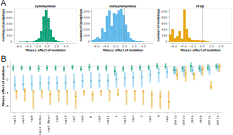
\includegraphics[width=\linewidth]{figs/dist.pdf}
\caption{
Distribution of effects of different types of mutations.
{\bf (A)}
Histograms of effects of synonymous, nonsynonymous, and stop-codon mutations across all viral genes.
Neutral mutations have effects of zero (dashed gray vertical lines), and deleterious mutations have negative effects.
{\bf (B)}
Effects of each type of mutation for each viral gene.
Dark squares indicate the median effect, and the lighter rectangles span the interquartile range.
Mutation types are color-coded as in panel A.
Both panels show only mutations with expected counts of at least 10.
See \url{https://jbloomlab.github.io/SARS2-mut-fitness/effects_histogram.html} and \url{https://jbloomlab.github.io/SARS2-mut-fitness/effects_dist.html} for interactive versions of these plots that allow adjustment of the expected-count cutoff and other options (such as separate histograms for each gene).
\label{fig:dist}
}
\end{figure*}

\begin{figure*}
\centering
\includegraphics[width=\linewidth]{figs/corr.png}
\caption{
Correlations between amino-acid fitness estimates made using different sequence subsets.
{\bf (A)} Estimates made using only sequences from the indicated viral clades, or {\bf (B)} estimates made using only sequences from the USA or England.
Each point is a different amino-acid mutation, and the orange text at upper left shows the number of mutations and Pearson correlation coefficient.
Both panels show only mutations with expected counts of at least 10 in each subset of sequences.
See \url{https://jbloomlab.github.io/SARS2-mut-fitness/clade_corr_chart.html} and \url{https://jbloomlab.github.io/SARS2-mut-fitness/subset_corr_chart.html}.For interactive versions of these plots that show correlations among additional clade pairs, allow adjustment of the expected-count cutoff, and allow examination of mutations for just specific genes.
\label{fig:corr}
}
\end{figure*}

\begin{figure*}
\centering
\includegraphics[width=0.75\linewidth]{figs/dms.png}
\caption{
Correlation of amino-acid fitness estimates with experimental measurements from deep mutational scanning studies for {\bf (A)} spike and {\bf (B)} Mpro (nsp5).
Each point is an amino-acid mutation, and the orange text in the upper left shows the number of mutations and Pearson correlation coefficient.
Data are taken from two independent deep mutational scanning studies for spike~\citep{cite}, and two studies for Mpro~\citep{cite}.
Each sub-panel shows a different set of mutations (depending on which mutations were measured in that experiment), and and only shows fitness estimates for mutations with at least 10 expected counts.
See \url{https://jbloomlab.github.io/SARS2-mut-fitness/dms_S_corr.html} and \url{https://jbloomlab.github.io/SARS2-mut-fitness/dms_nsp5_corr.html} for interactive versions of these plots that enable subsetting on just mutations shared across all datasets, and adjustment of the minimum expected count cutoff .
\label{fig:dms_corr}
}
\end{figure*}

\begin{figure*}
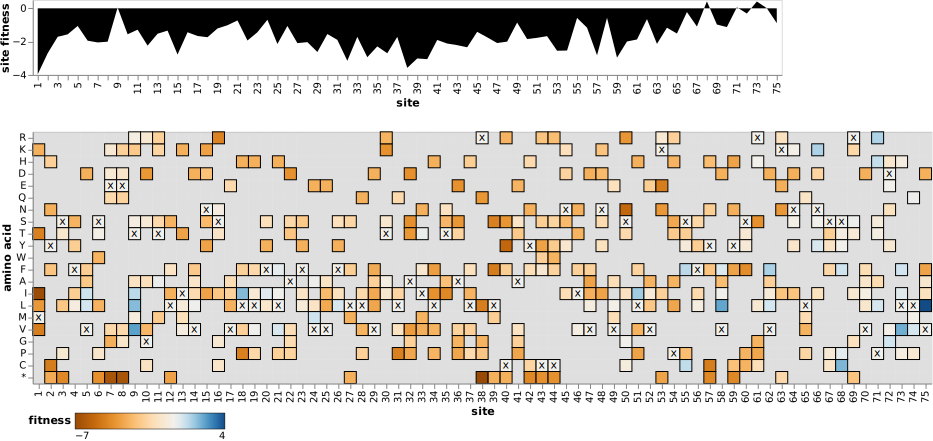
\includegraphics[width=\linewidth]{figs/E_heatmap.pdf}
\caption{
Effects of amino-acid mutations to E protein.
The area plot at top shows the average effects of mutations at each site, and the heatmap shows the effects of specific amino acids, with \textbf{x} denoting the amino-acid identity in the Wuhan-Hu-1 strain.
Only mutations with at least 10 expected counts are shown.
See \url{https://jbloomlab.github.io/SARS2-mut-fitness/E.html} for an interactive version of this plot that enables zooming, mouseovers, and adjustment of the minimum expected count threshold.
See the links at \url{https://jbloomlab.github.io/SARS2-mut-fitness} for comparable interactive plots for all other SARS-CoV-2 proteins.
\label{fig:E_heatmap}
}
\end{figure*}

\begin{figure*}
\centering
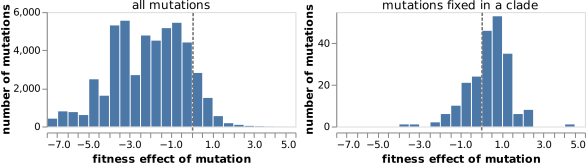
\includegraphics[width=0.7\linewidth]{figs/fixed_dist.pdf}
\caption{
Distribution of fitness effects of all amino-acid mutations relative to Wuhan-Hu-1, and all mutations that fixed in at least one clade of SARS-CoV-2 (using the Nextstrain clade definitions).
The vertical dashed line at zero indicates the effect of a neutral mutation.
Estimates are only shown for mutations with expected counts of at least 10.
See \url{https://jbloomlab.github.io/SARS2-mut-fitness/clade_fixed_muts_hist.html} for an interactive version of this plot that allows adjustment of the minimum expected count threshold.
\label{fig:fixed_dist}
}
\end{figure*}

\section{Discussion}


{\small

\section{Methods}
\subsection{Code and data availability}
Code and data are at \url{https://github.com/jbloomlab/SARS2-mut-fitness}.

\section{Acknowledgments}
We thank Angie Hinrichs for assistance with resolving several questions related to use of the UShER package and its pre-built mutation-annotated tree \jdbcomment{if we don't add as co-author}.
\jdbcomment{Jesse to acknowledge AVIDD, CEIRR, and R01 grants.}
JDB is an Investigator of the Howard Hughes Medical Institute.

\section{Competing interests}
JDB is on the scientific advisory boards of Apriori Bio, Aerium Therapeutics, Invivyd, the Vaccine Company, and Oncorus.
JDB receives payments as an inventor on a Fred Hutch licensed patents related to deep mutational scanning of viral proteins.

\bibliography{references}
}

\onecolumn
\renewcommand{\thepage}{S\arabic{page}}
\setcounter{page}{1}
\renewcommand{\thefigure}{S\arabic{figure}}
\setcounter{figure}{0}

\clearpage

\section{Supplementary Material}

\begin{figure*}[b]
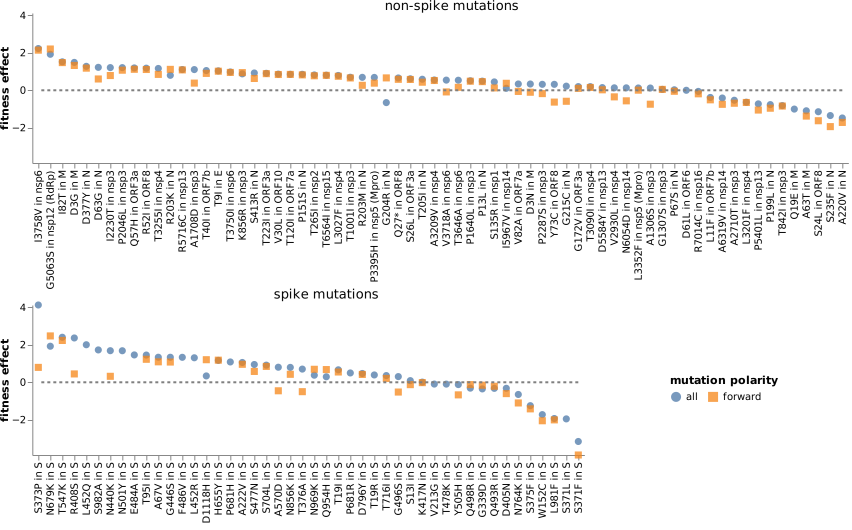
\includegraphics[width=\linewidth]{figs/fixed.pdf}
\caption{
Effects of individual mutations that fixed in at least one clade of SARS-CoV-2, faceted by whether they are in spike or another protein.
Plots show estimates of effects of mutations made across all clades (including those that have fixed the mutation) and just from direct forward occurrences of the mutation in clades in which it has not yet fixed.
Estimates are only shown for mutations with expected counts of at least 10.
See \url{https://jbloomlab.github.io/SARS2-mut-fitness/clade_fixed_muts.html} for an interactive version of this plot.
\label{fig:fixed}
}
\end{figure*}


\begin{figure*}
\centering
\includegraphics[width=0.75\linewidth]{figs/terminal.png}
\caption{
Relationship between fitness effects of mutations and ratio of counts on terminal (tip) branches versus non-terminal (internal) branches.
Each point is an amino-acid mutation, and the orange text in the upper left give the number of mutations and the Pearson correlation coefficient.
This plot shows only mutations with at least 10 expected counts and 5 actual counts.
See \url{https://jbloomlab.github.io/SARS2-mut-fitness/fitness_vs_terminal.html} for an interactive version of this plot that allows filtering by the number of actual or expected counts, or by gene.
\label{fig:terminal}
}
\end{figure*}

\end{document}
